\section{Aufgenommene Datenmenge}
\label{sec:DymelData}
\texttt{DymelData} ist eine Datenmenge, die mit dem \texttt{Recorder} (siehe Sektion \ref{sec:recorder}) erstellt wurde. Sie umfasst insgesamt 14410 Gesten in unterschiedlichen Konfigurationen. Die Datenmenge wurde
einerseits aufgenommen, um unter den vorort bestehenden Lichtverhältnissen die Modelle miteinander vergleichen zu können und andererseits, um Test- und Trainingsdaten für Nullgesten bereitzustellen. In den
bisherigen Datenmengen ist nur ein geringer Anteil an Nullgesten enthalten.
\newline
\newline
\subfigbox{
\subfigure[Geringe Helligkeit]{\label{subfig:light_low}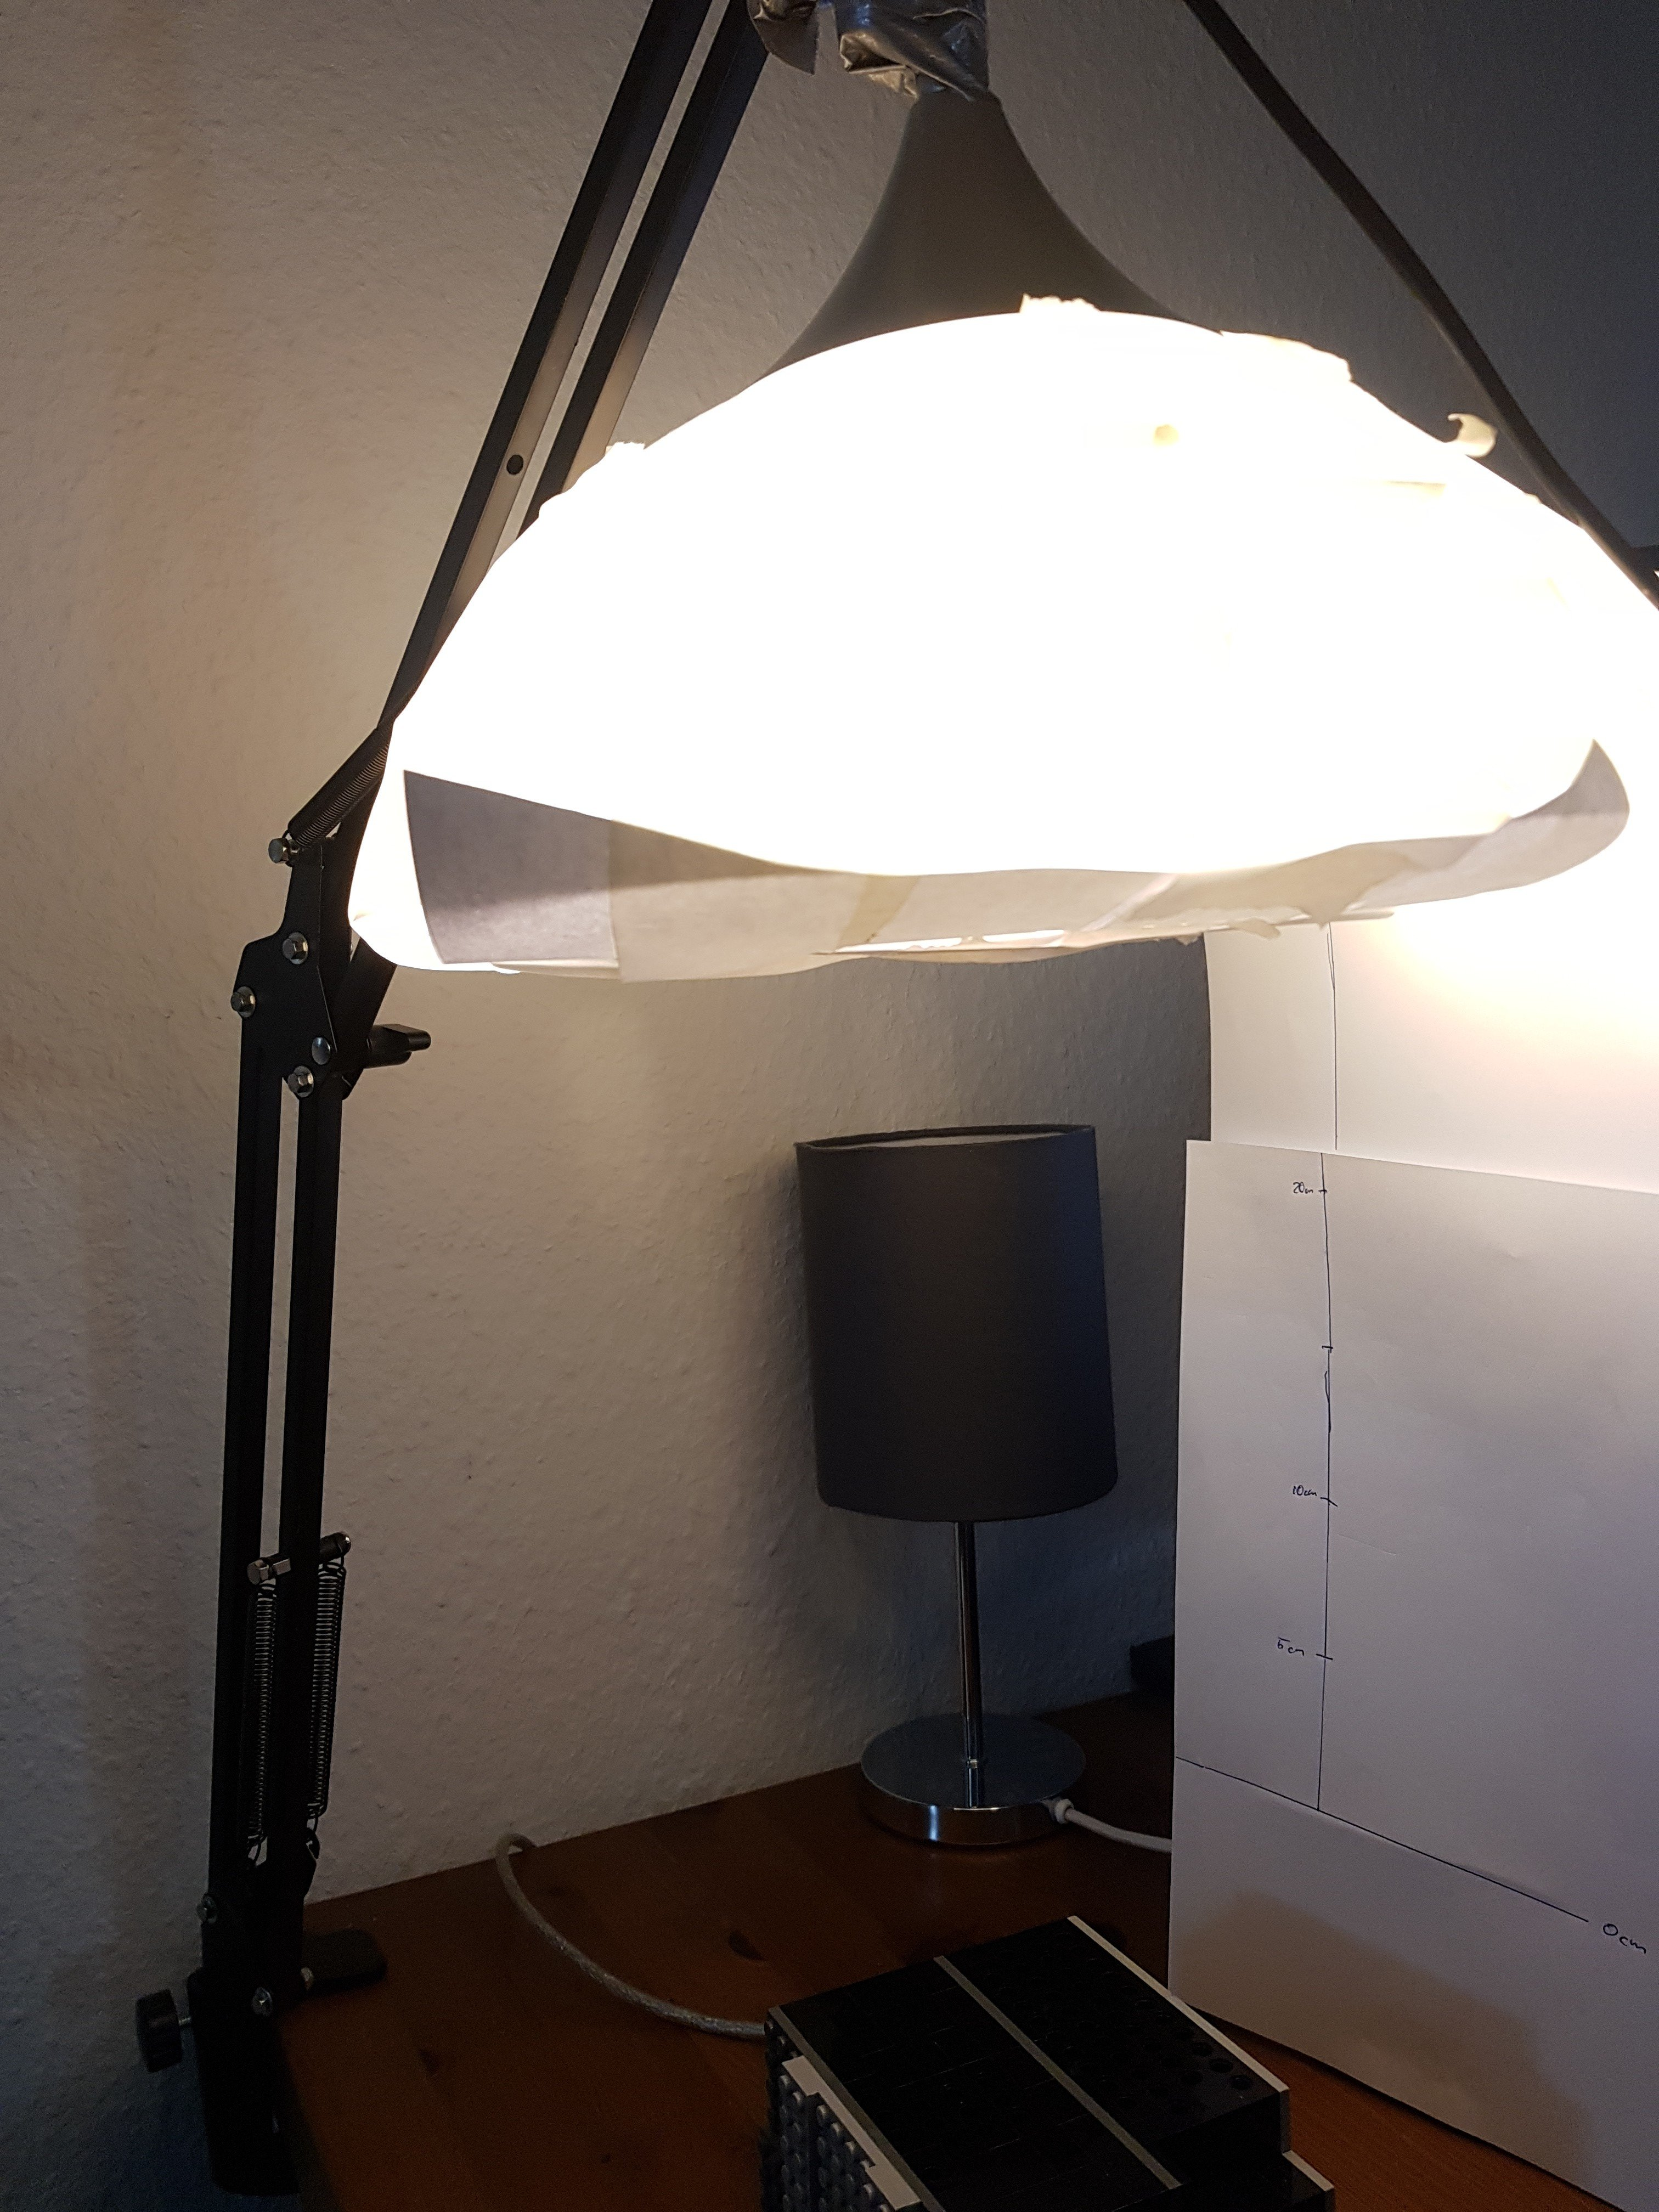
\includegraphics[width=0.33\linewidth]{images/light_low.jpeg}}\hfill%
\subfigure[Halbe Helligkeit]{\label{subfig:light_medium}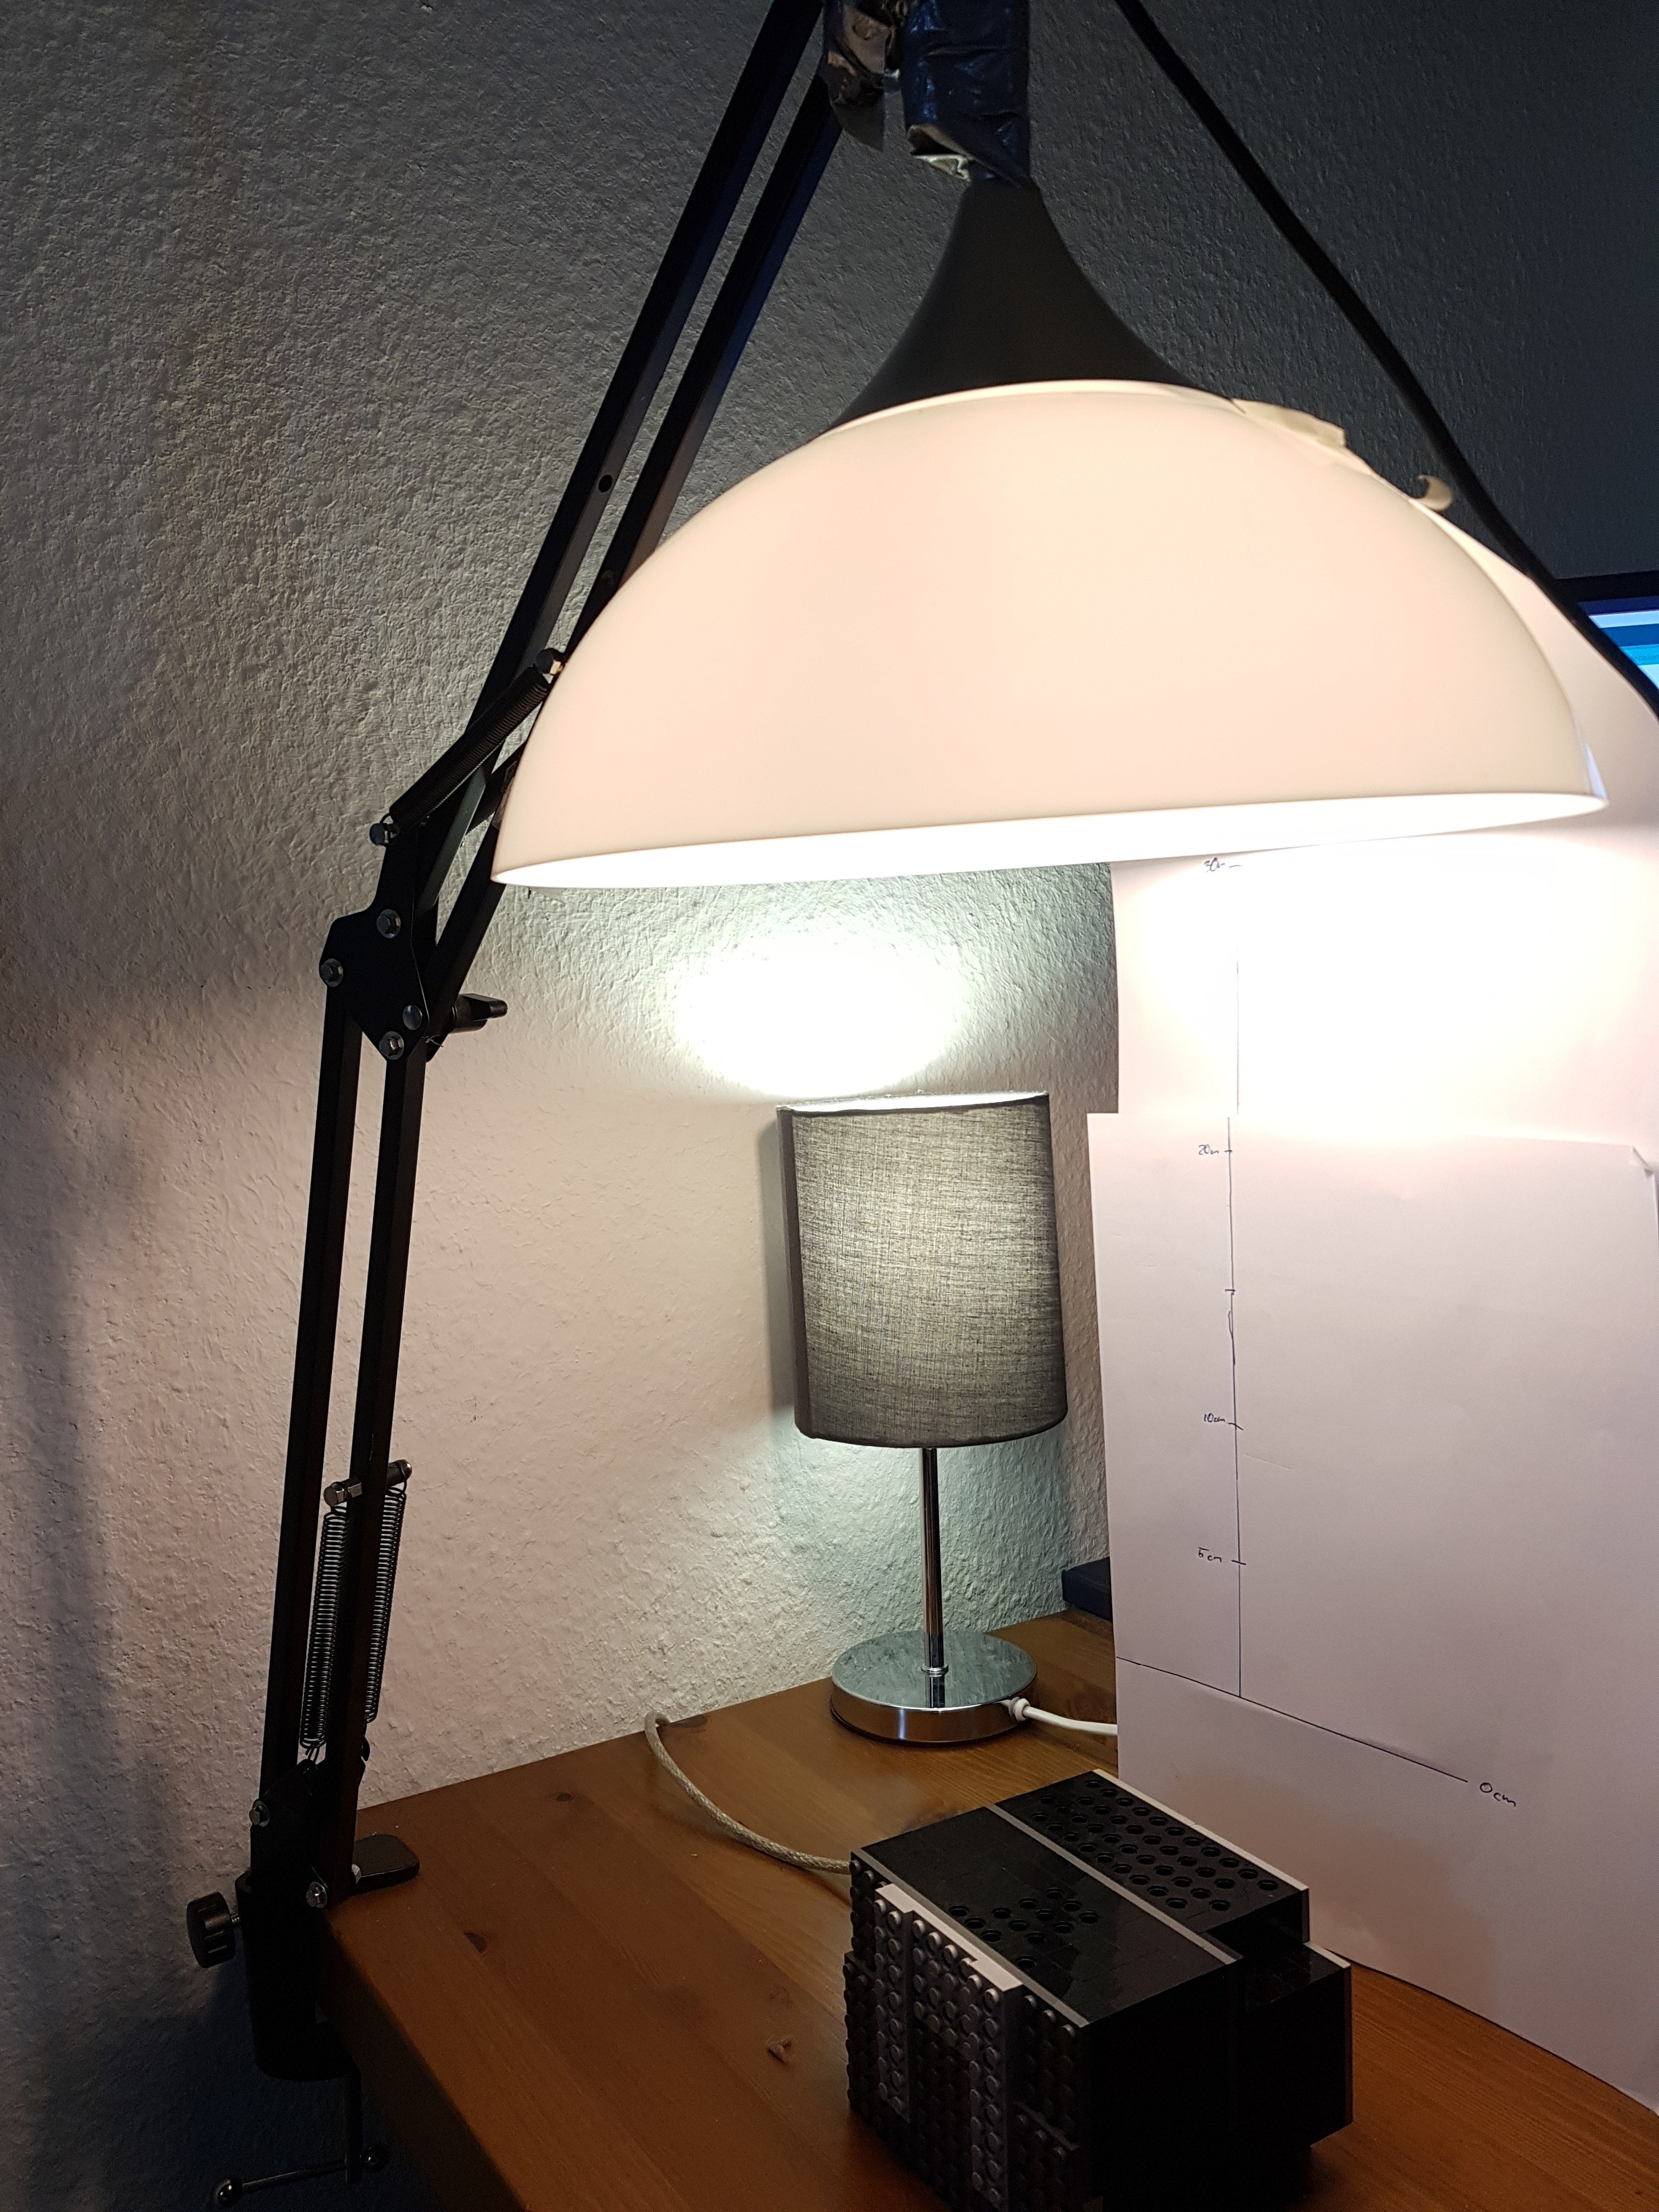
\includegraphics[width=0.33\linewidth]{images/light_medium.jpeg}}\hfill%
\subfigure[Hohe Helligkeit]{\label{subfig:light_high}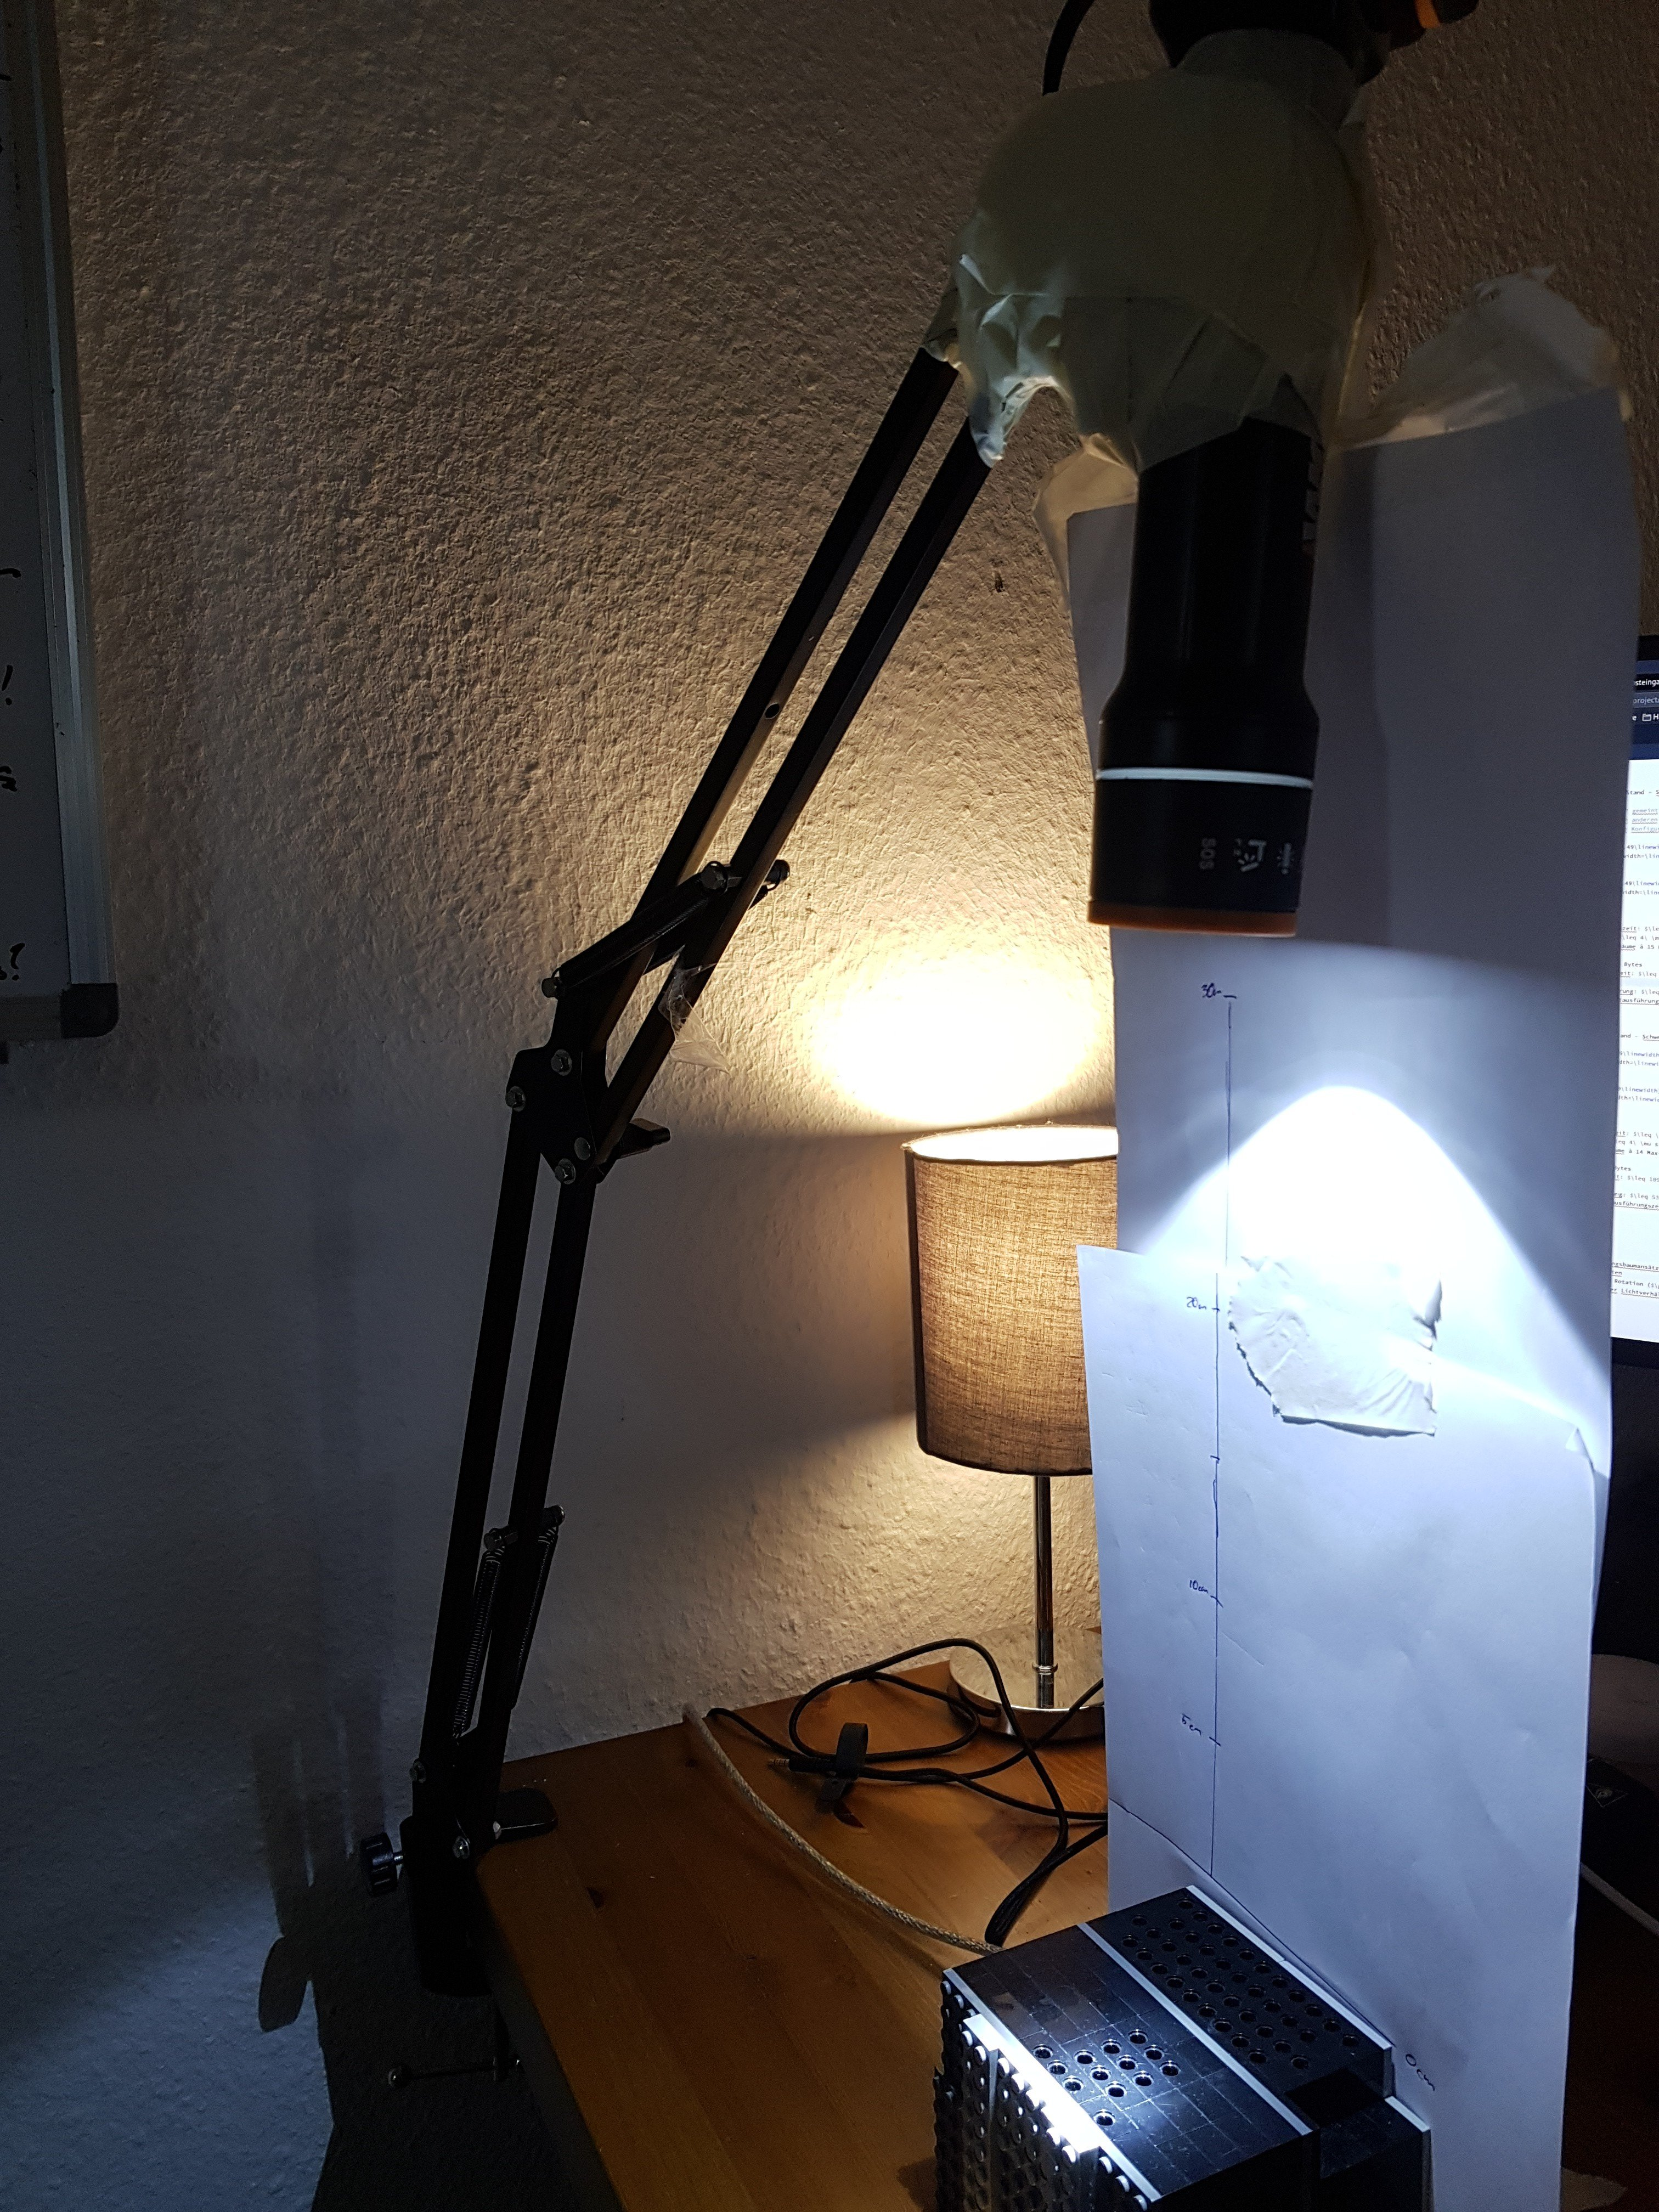
\includegraphics[width=0.33\linewidth]{images/light_high.jpeg}}%
}{Verschiedene Helligkeitsstufen unter denen die Gesten von \texttt{DymelData} aufgenommen wurden.}{fig:different_lights}
Jede Handgeste wurde unter jeder Konfiguration ca. 100 mal aufgenommen bei 90 Bildern pro Sekunde. Insgesamt wurden in 3 Lichtverhältnissen und 4 Distanzen, 6 verschiedene Gesten (Links nach Rechts,
Rechts nach Links, Oben nach Unten, Unten nach Oben und 2 Nullgesten) jeweils schnell und langsam aufgenommen. Die Handgesten wurden in den Abständen 5 cm, 10 cm, 20 cm und 25 cm aufgenommen.
\newline
\newline
Die \glqq Geringe\grqq\ Helligkeit war im Durchschnitt bei ca. 140, \glqq Halbe\grqq\ Helligkeit bei ca. 659, \glqq Hohe\grqq\ Helligkeit bei ca. 908. Alle Helligkeiten haben das 3x3-Array
relativ gleichmäßig ausgeleuchtet. Bei den Lichtquellen \ref{subfig:light_low} und \ref{subfig:light_medium} wurde eine Schirmlampe verwendendet. Dadurch wurde das Licht relativ breit gestreut,
wodurch mit zunehmender Distanz der Kontrast abgenommen hat. Bei \ref{subfig:light_high} wurde eine Punktlichtquelle verwendet, wodurch der Kontrast über alle Distanzen sehr stark ist.
Im weiteren Verlauf dieser Arbeit wird diese Datenmenge ohne Nullgesten \glqq Gestenmenge\grqq\ genannt. Die ersten 25\% werden zum Trainieren verwendet, die hinteren 75\% zum Testen. Die Testmenge
wird im weiteren \glqq Gestentestmenge\grqq\ genannt.
\newline
\newline
Insgesamt wurden 2 Typen von Nullgesten aufgenommen. Die erste Nullgeste geht \textit{Oben} rein, verschieden weit in Richtung \textit{Unten} und kehrt anschließend um, um bei \textit{Oben} wieder rauszukommen.
Die zweite Nullgeste geht \textit{Oben} rein, verschieden weit in Richtung \textit{Unten} und anschließend \textit{Rechts} wieder raus. Die resultierenden Handgesten werden anschließend um 90°, 180° und
270° rotiert, um die equivalenten Nullgesten aus den anderen Richtungen zu inferieren. Insgesamt enstehen dadurch 19400 Nullgesten. Im weiteren Verlauf dieser Arbeit wird diese Datenmenge mit auschließlich
Nullgesten \glqq Nullgestenmenge\grqq\ genannt. Die ersten 12,5\% werden zum Trainieren verwendet, die hinteren 87,5\% zum Testen. Die Testmenge wird im weiteren \glqq Nullgestentestmenge\grqq\ genannt.
\newline
\newline
Um zu testen wie gut das Model sich gegenüber verschiedene Lichtverhältnisse generalisiert hat, ist es nötig mehr als nur 3 Helligkeitsstufen zu testen. Aus diesem Grund wurde aus dem Anteil der Gestenmenge mit
der Helligkeit \glqq Gering\grqq\ eine synthetische Testmenge generiert. Dabei wurden jeweils 16 Duplikate der Datenmenge erstellt mit einem Helligkeitsoffset zwischen 50 und 800 und einer
Skalierung zwischen 1 und 7. Diese Datenmengen wurden zu einer Testmenge zusammengefügt. Im weiteren Verlauf dieser Arbeit wird diese Testmenge \glqq Helligkeitstestmenge 1\grqq\ genannt.
\newline
\newline
Zusätzlich zu einer Testmenge, die den Kontrast immer weiter erhöht, bedarf es eine Testmenge, die bei gleichbleibender Helligkeit den Kontrast verringert. Aus diesem Grund wurde aus dem Anteil der Gestenmenge mit
der Helligkeit \glqq Medium\grqq\ eine synthetsiche Testmenge generiert. Dabei wurden 19 Duplikate erstellt, die in $0,05$ Schritten die Helligkeit runterskalieren. In jedem Schritt wird in gleichen
Anteilen die Gesamthelligkeit auf jeden Pixel addiert. Dadurch wird der Kontrast zwischen dunklen und hellen Pixeln immer geringer. Im weiteren Verlauf dieser Arbeit wird diese Testmenge
\glqq Helligkeitstestmenge 2\grqq\ genannt.